\documentclass[11pt,a4paper]{article}
\usepackage[UTF8]{ctex}
\usepackage[a4paper,left=25mm,right=25mm,top=22mm,bottom=22mm]{geometry}
\usepackage{fontspec,xeCJK,graphicx,amsmath,amssymb}
\usepackage[hidelinks]{hyperref}
\setmainfont{Times New Roman}
\setCJKmainfont{SimSun}[BoldFont=SimHei]
\setCJKsansfont{SimHei}
\setlength{\parindent}{2em}
\setlength{\parskip}{3pt}
\linespread{1.18}
\emergencystretch=1em
\widowpenalty=10000
\clubpenalty=10000
\setlength{\textfloatsep}{10pt}
\setlength{\intextsep}{10pt}
\setlength{\abovecaptionskip}{5pt}
\renewcommand{\topfraction}{0.9}
\renewcommand{\bottomfraction}{0.9}
\renewcommand{\textfraction}{0.08}
\renewcommand{\floatpagefraction}{0.8}
\graphicspath{{../figures/eda-v2/}}
\makeatletter
\newenvironment{inlinefigure}{\par\addvspace{10pt}\noindent\begin{minipage}{\linewidth}\def\@captype{figure}\centering}{\end{minipage}\par\addvspace{10pt}}
\makeatother
\pagestyle{plain}
\begin{document}

\section*{7 数据整理与特征分析}

\subsection*{7.1 数据来源与整理}

题目给出的数据分别描述了一天的参考供需、全年实际运行情况，以及运行中不断更新的光伏预报。附件1包含一天内144个时刻的负载、光伏预测和电价，相邻记录间隔10分钟。附件2给出2025年1月1日至12月31日的实际负载与光伏功率，共52560组记录；附件4提供同期、同样间隔的电价。附件3则在每天0、6、12和18点各发布一次光伏预报，每次给出未来24个整点的预测值，全年共35040条。附件5为各问的结果填写格式。

每天零点制定购电计划时，当天的实际负载和光伏出力还不清楚。因此，问题二需要参考此前的运行记录判断当天供需；问题三还可以使用零点发布的光伏预报，并在白天收到新预报后重新判断。按本文采用的设定，问题四的未来电价同样需要提前估计。虽然附件保存了全年实际值，这些数值在每日运行过程中仍是随时间逐步出现的。以下全年统计用于了解数据的整体特点，具体日期的计划则依据该日决策时已有的记录制定。

原始表格中的日期和时间有多种写法。整理时将它们转换为统一格式，并保留原有日期、时间和对应数值。例如，末行的“0:00+1”表示次日零点，应与当日零点分开记录。负载、光伏和电价按原表相同的日期与时刻对应起来；预报表中同组共用的日期补记到各行，同时保留预报的发布时间和所预测的时刻。这样，同一个未来时刻在零点、6点等不同时间得到的预报都能分别找到，较早的预报也不会被后来的版本覆盖。

整理后的数据与原表逐项比对，数值保持一致，所用数值列没有空值、无穷值或负值。本次整理保留了光伏零值和电价极值，没有对它们进行替换、平滑或删减。功率仍以kW表示，电价以元/kWh表示；本节的日均、月均功率均由相应采样值取算术平均得到。功率表示某一时刻的供需水平，电量则要结合持续时间计算，二者分别用于观察供需变化和核算购电、储能使用。

\subsection*{7.2 一天内的供需错配}

将附件1的负载、光伏预测和电价放在一起，可以看到三者的高峰并不同时出现。负载在9:10达到5958.97 kW，光伏则在12:10达到7612.32 kW。图\ref{fig:reference}进一步给出负载减去光伏后的功率差：正值表示还需要外网或电池补充供电，负值表示光伏在满足当时负载后仍有富余。

\begin{inlinefigure}
  \centering
  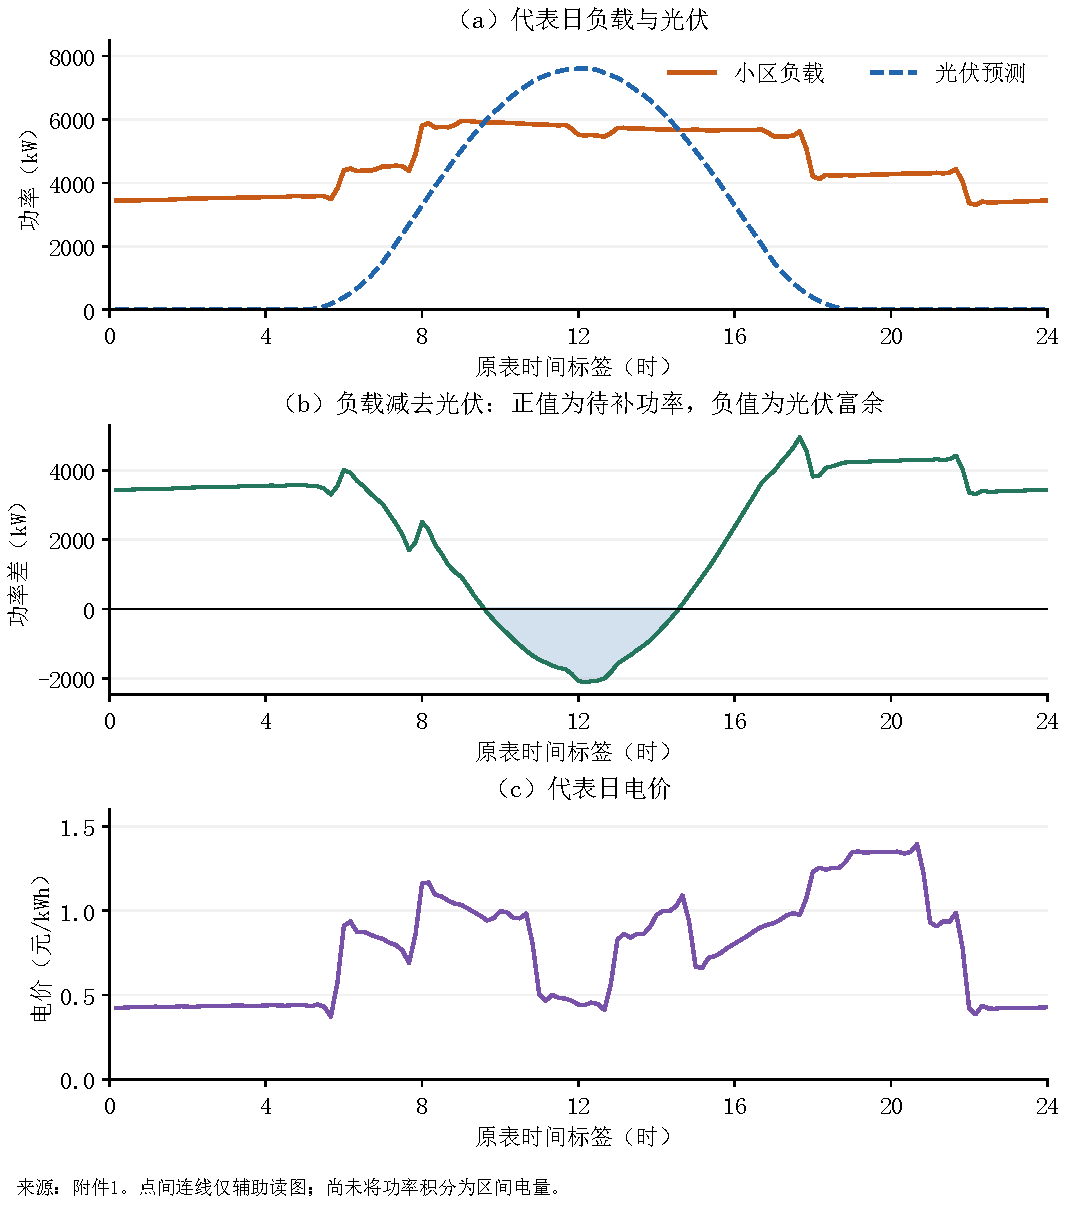
\includegraphics[width=0.90\linewidth]{01_reference_day.pdf}
  \caption{代表日负载、光伏预测、功率差与电价的日内变化}
  \label{fig:reference}
\end{inlinefigure}

9:40至14:30的连续30个记录中，光伏均超过负载，最大富余功率为2117.53 kW；到17:40，负载与光伏的差额又达到4956.50 kW。与此同时，电价在5:40最低，为0.3713元/kWh，在20:40最高，为1.3952元/kWh。午间剩下的电与傍晚需要的电存在时间差，储能可以连接这两个时段。低价时提前购电充电也有利用价值，但能够转移多少电量、转移后是否节省费用，还取决于储能容量、充放电功率和损耗。

附件1的曲线与全年各日相同时刻的平均曲线十分接近，但平均曲线会弱化具体日期的高峰。例如，全年实际负载最高达到7978.88 kW，高于代表日的5958.97 kW。全年还有330天出现过光伏超过负载的记录，这类记录占全部采样点的19.27\%。这些富余电力能否留到以后使用，要看当时电池还能接收多少；19.27\%描述的是出现富余的采样点比例，实际未利用电量还需结合储能运行计算。

\subsection*{7.3 年内的供需变化}

图\ref{fig:annual}将全年每天的平均负载、光伏功率和电价与各月平均水平放在一起。逐日曲线保留短期起伏，月均曲线显示较缓慢的变化。7月平均负载最高，为5337.26 kW；光伏月均功率则在8月最高，为2915.99 kW，到12月降至1513.84 kW。不同月份的发电和用电变化并不同步。

\begin{inlinefigure}
  \centering
  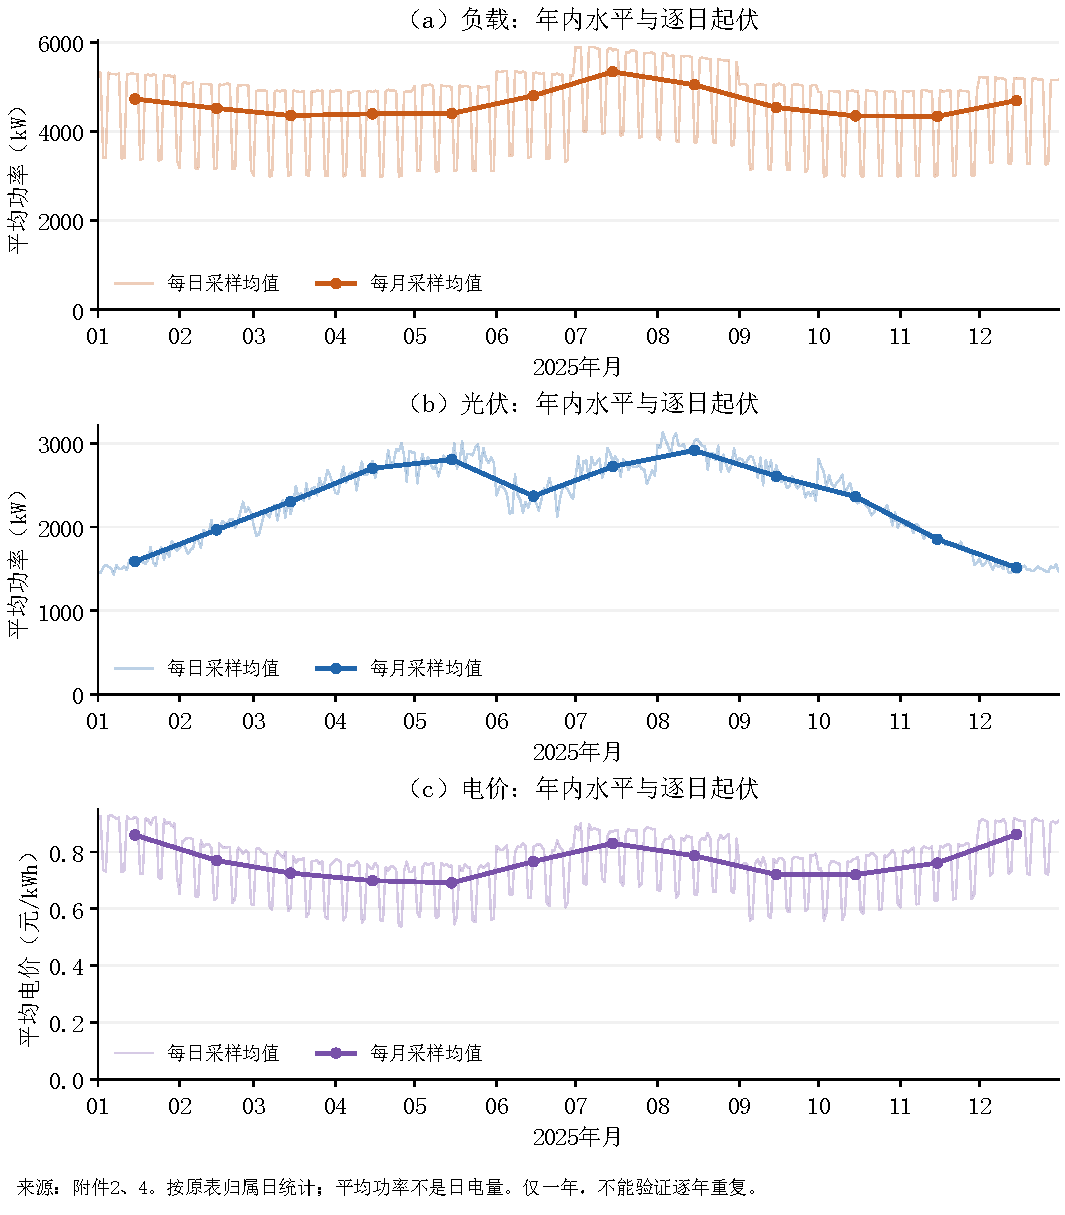
\includegraphics[width=0.90\linewidth]{02_year_and_month.pdf}
  \caption{2025年负载、光伏功率和电价的逐日均值与月均值}
  \label{fig:annual}
\end{inlinefigure}

这种差异使得负载最高的月份未必有最大的供需差额。12月平均负载为4691.31 kW，低于7月，但同期光伏较少，平均负载减光伏达到3177.47 kW，高于7月的2614.00 kW，约为5月1595.18 kW的两倍。冬季即使平均负载没有达到全年高峰，仍可能更依赖外网补充。判断供电压力时，需要同时看负载和光伏，单独观察用电高低容易遗漏这一变化。

光伏在年内也并非平滑变化：6月平均功率为2369.83 kW，低于相邻的5月和7月。由于附件没有提供对应天气资料，这一回落暂不能归因于某种气象原因。现有数据说明2025年存在明显的季节差异；只有一年的记录，尚不足以判断这些差异在其他年份是否以同样方式重复。

\subsection*{7.4 星期差异与电价波动}

将负载序列与一天前、一周前的序列比较，相关系数分别为0.6792和0.9855，同一星期位置的负载更为相似。扣除各月相同时刻的平均水平后，一周间隔的相关系数仍为0.9800，说明每周重复的特点并非仅来自每天共同的高低起伏。

按原表日期统计，周五、周六的平均负载为3265.40 kW，比其余五天的5168.20 kW低约36.82\%，平均电价也较低，如图\ref{fig:prices}所示。这种星期差异在各月均可观察到，因而参考历史供需时，除前一天的情况外，同一星期位置的记录也值得关注。

\begin{inlinefigure}
  \centering
  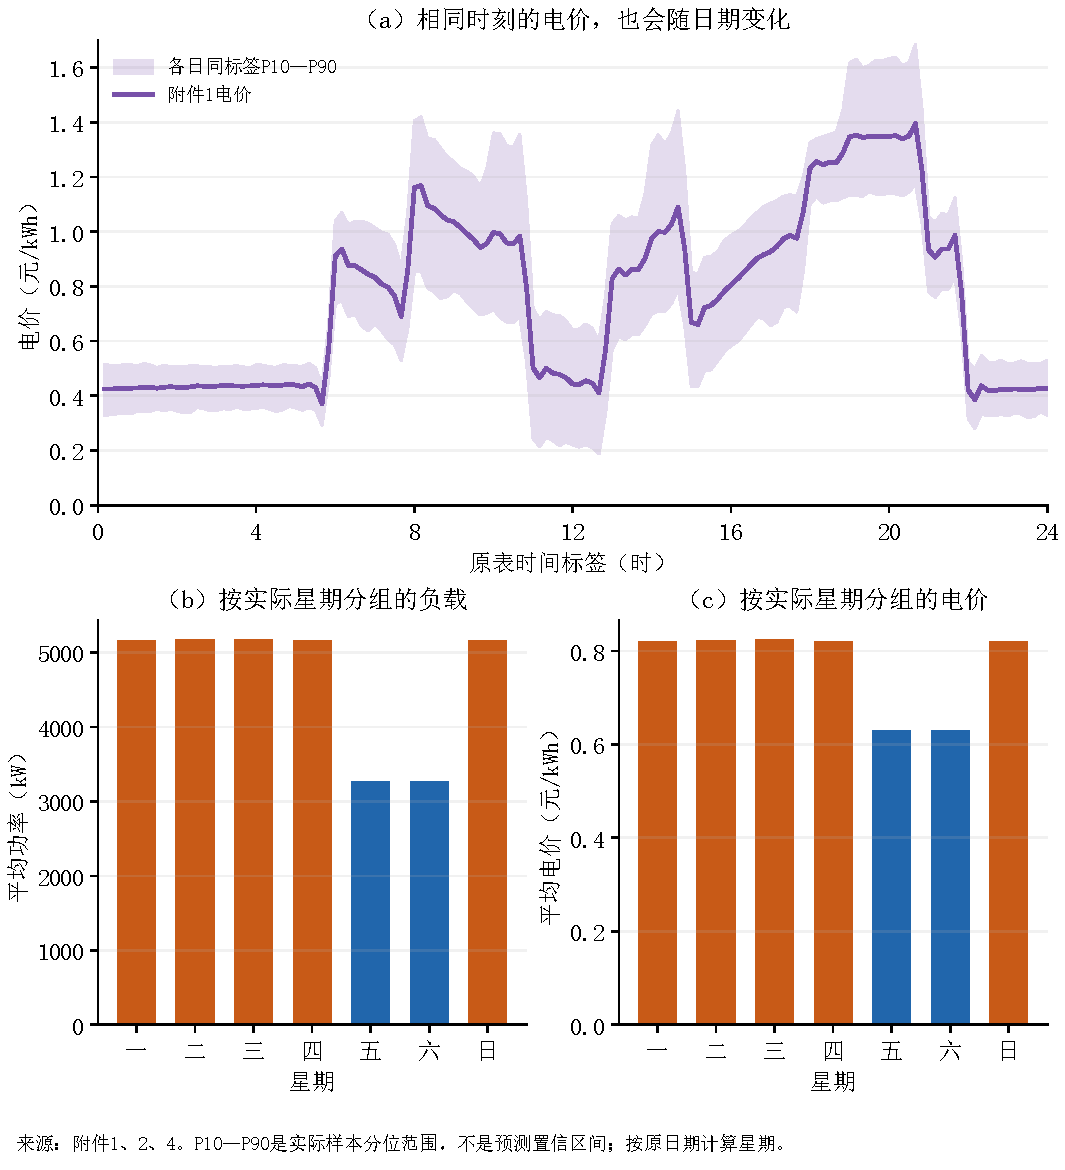
\includegraphics[width=0.86\linewidth]{06_prices_and_weekdays.pdf}
  \caption{日内电价的跨日变化范围及各星期的平均负载、电价}
  \label{fig:prices}
\end{inlinefigure}

光伏序列相隔一天和一周的相关系数都接近0.99，但扣除各月相同时刻的平均水平后，一周间隔的相关系数降至$-0.0148$。原有的高相关主要反映白天发电、夜间接近零的共同形状，尚未显示出与负载同样强的独立周规律。

电价的一周间隔相关系数在上述处理后为0.8489，也有较强的周变化。图\ref{fig:prices}中的阴影表示全年同一时刻实际价格的第10至第90百分位范围，体现出固定日内电价未能反映的跨日波动。全年价格介于0.0076至1.7936元/kWh，按天计算的最高价与最低价之比的中位数为4.33。这些变化会影响提前购电和储能使用的收益，也使问题四需要在未来价格尚不确定时权衡买电时机。

\subsection*{7.5 光伏预报的误差与更新}

为了解光伏预报的偏差，将附件3的预报与附件2中同一目标整点的实测功率对应。35040条预报中，35004条有实测值，其余36条预测的时刻超出实际数据末端，因此保留记录而不参与误差计算。以下直接比较整点值，没有插值为10分钟序列。

将预报与实测的绝对差取平均，得到平均绝对误差。全部匹配记录的误差为186.61 kW，实测光伏大于零的记录则为373.28 kW，可见夜间零值会降低总体平均误差。在实际有光伏的记录中，提前1小时和24小时预报的误差分别为37.37 kW和750.09 kW。图\ref{fig:forecast}呈现出提前越久、偏差总体越大的特点，不过各提前量包含的目标时刻并不完全相同。

\begin{inlinefigure}
  \centering
  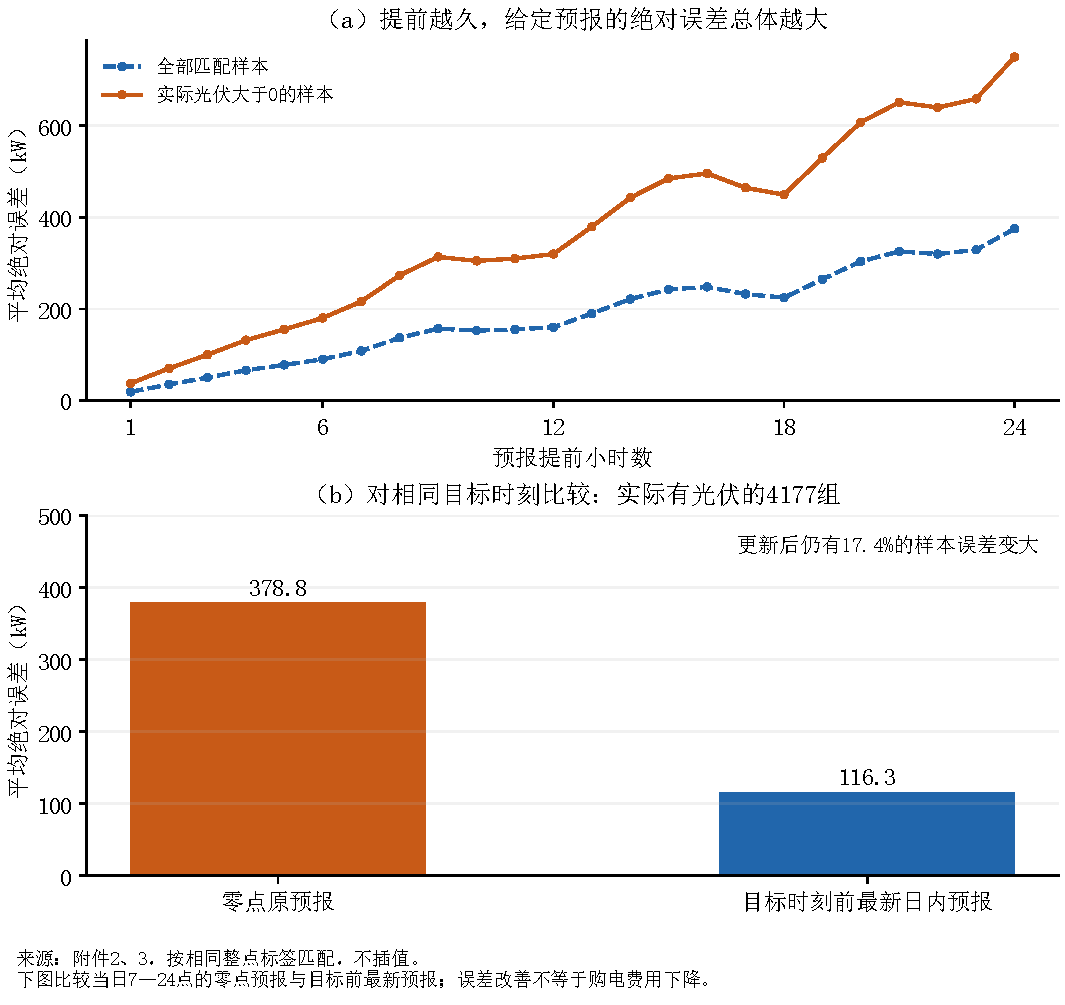
\includegraphics[width=0.86\linewidth]{07_forecast_accuracy.pdf}
  \caption{不同提前量的光伏预报误差及同一目标时刻的更新比较}
  \label{fig:forecast}
\end{inlinefigure}

再对每天7点至24点的同一目标时刻，分别取零点预报和目标发生前已发布的最新预报，共得到6570组配对。其中4177组的实测光伏大于零，更新后的平均绝对误差由378.79 kW降至116.30 kW，下降69.30\%；81.54\%的配对误差减小，17.43\%增大，其余不变。按实测光伏是否大于零分组，有助于事后看清发电时的误差，但制定计划时尚不能知道哪些记录会落入这一分组。

日内更新总体上提供了更准确的信息，但并非每次都更准确。即使新预报更接近实际，也未必值得立即修改计划：原计划的偏差可能由电池吸收，修改合同还会产生费用。因此，预报误差的下降能否转化为购电费用的下降，仍需在第三问中结合储能状态和调整费用判断。

\end{document}
